\documentclass{VUMIFPSkursinis}
\usepackage{algorithmicx}
\usepackage{algorithm}
\usepackage{algpseudocode}
\usepackage{amsfonts}
\usepackage{amsmath}
\usepackage{bm}
\usepackage{caption}
\usepackage{color}
\usepackage{float}
\usepackage{graphicx}
\usepackage{listings}
\usepackage{subfig}
\usepackage{wrapfig}

\usepackage{enumitem}
%PAKEISTA, tarpai tarp sąrašo elementų
\setitemize{noitemsep,topsep=0pt,parsep=0pt,partopsep=0pt}
\setenumerate{noitemsep,topsep=0pt,parsep=0pt,partopsep=0pt}

% Titulinio aprašas
\university{Vilniaus universitetas}
\faculty{Matematikos ir informatikos fakultetas}
\department{Programų sistemų katedra}
\papertype{Laboratorinis darbas}
\title{Muzikos kaupimo programos MuziX projektas}
\titleineng{A project for a music hoarding program MuziX}
\status{2 kurso 5 grupės studentai}
\author{Goda Radlinskaitė, Gabrielė Žielytė}
\secondauthor{Valdas Rakutis, Nedas Valentinovičius}   % Pridėti antrą autorių

\supervisor{dr. Vytautas Valaitis}
\date{Vilnius – \the\year}

% Nustatymai
\setmainfont{Palemonas}   % Pakeisti teksto šriftą į Palemonas (turi būti įdiegtas sistemoje)
\bibliography{bibliografija}

\begin{document}
	
% PAKEISTA	
\maketitle
\cleardoublepage\pagenumbering{arabic}
\setcounter{page}{2}

%TURINYS
\tableofcontents

\sectionnonum{Įvadas}
Šio darbo tikslas yra suprojektuoti intuityvią, naudotojui aiškią ir nesunkiai naudojamą, greitai veikiančią muzikos kaupimo programą. Ši programa naudotojo pateiktą nuorodą į muzikinį kūrinį prideda į jo sudarytus grojaraščius ir leidžia jų klausytis ne tik platformoje, kurioje buvo įvykdytas kūrinio pasirinkimas, bet ir kitose platformose ar įrenginiuose. MuziX veiks Windows bei Android operacinėse sistemose, vartotojui prisijungus prie savo paskyros jo dainos bei grojaraščiai bus randami visuose programą palaikainčiuose įrenginiuose.

MuziX programa yra išskirtinė tuo, kad padaro tai, ko kitos šiuo metu egzistuojančios muzikos klausymo platformos nesugeba įgyvendinti ar įgyvendina limituotai - kaupti savąją dainų kolekciją iš įvairių šaltinių. Kai kurios platformos už jų siūlomos muzikinės bibliotekos papildymą pačių programos naudotojų turimais kūriniais prašo mėnesinių mokesčių ar yra išvis draudžiamos Lietuvoje bei daugelyje kitų šalių. Šis projektas bando pašalinti šiuos limitus, leisdamas nesunkiai kurti savą muzikos kolekciją be papildomų mokesčių ar draudimų.

Šiuo projektu siekiama palengvinti muzikos megėjų, saugančių savo muzikinę kolekciją daugybėje skirtingų vietų, gyvenimus leidžiant jiems apjungti įvairius muzikos ar kitų garso takelių šaltinius. Tikimasi, kad galų gale MuziX bus pagrindinė bei mėgiamiausia ne tik Lietuvių, bet ir kitų šalių gyventojų muzikinė platforma.


\section{Informacija apie projektą}
Medžiagos darbo tema dėstymo skyriuose pateikiamos nagrinėjamos temos detalės:
pradinė medžiaga, jos analizės ir apdorojimo metodai, sprendimų įgyvendinimas,
gautų rezultatų apibendrinimas. Šios dalies turinys labai priklauso nuo darbo
temos. Skyriai gali turėti poskyrius ir smulkesnes sudėtines dalis, kaip
punktus ir papunkčius.

Medžiaga turi būti dėstoma aiškiai, pateikiant argumentus. Tekstas dėstomas
trečiuoju asmeniu, t.y. rašoma ne „aš manau“, bet „autorius mano“, „autoriaus
nuomone“. Reikėtų vengti informacijos nesuteikiančių frazių, pvz., „...kaip jau
buvo minėta...“, „...kaip visiems žinoma...“ ir pan., vengti grožinės literatūros
ar publicistinio stiliaus, gausių metaforų ar panašių meninės išraiškos
priemonių.

\subsection{Programos paskirtis}
%Citavimo pavyzdžiai: cituojamas vienas šaltinis \cite{PvzStraipsnLt}; cituojami
%keli šaltiniai \cite{PvzStraipsnEn, PvzKonfLt, PvzKonfEn, PvzKnygLt, PvzKnygEn,
%PvzElPubLt, PvzElPubEn, PvzMagistrLt, PvzPhdEn}.
MuziX - tai programa, skirta muzikos iš įvairių šaltinių kaupimui ir klausymuisi, veikianti Windows bei Android operacinėse sistemose. Naudodama duomenų bazę, ji leidžia naudotojams prisijungti ir gauti prieigą prie savo muzikinės kolekcijos iš bet kurio įrenginio su įdiegta MuziX programėle. Pagrindinės autorių numatomos funkcijos yra šios:
\begin{itemize}
	\item Pridėti dainas į pagrindinį bei savo kurtus grojaraščius vieno mygtuko paspaudimu
	\item Sklandžiai ir neapkraunant įrenginio groti aukščiausios įmanomos kokybės muzikinius kūrinius
	\item Laikant informaciją apie naudotojus internetinėje duombazėje, leisti jiems prieiti savo saugomus kūrinius iš bet kurio įrenginio su MuziX programėle
\end{itemize}

\subsection{Pranašumai ir trūkumai}
Autoriai siekia, kad ši programa būtų pagrindinė muzikos klausymo platforma daugeliui žmonių. Tai norima pasiekti pateikiant tai, ko kitos muzikos klausymo platformos šiuo metu nesiūlo - neribotą ir nemokamą priėjimą prie muzikinės kolekcijos, sukauptos iš kelių šaltinių, leidžiančių trečios šalies programoms prieiti prie juose saugomų įrašų. Tokia idėja turi tam tikrų pranašumų ir trūkumų.
\subsubsection{Pranašumai}
\begin{itemize}
	\item Itin didelė muzikos šaltinių įvairovė
	\item Neribotas prieinamumas iš įvairių įrenginių
	\item Paprasta, greita, suprantama naudojimos aplinka
\end{itemize}
\subsubsection{Trūkumai}
\begin{itemize}
	\item Reikalingas nuolatinis interneto ryšys, nes įrašai grojami tiesiai iš šaltinių
	\item Vartotojai yra atsakingi už tai, kad jų naudojami šaltiniai leistų klausymąsi per trečios šalies programinę įrangą
\end{itemize}

%\begin{enumerate}
%	\item Pirmas elementas
%	\item Antras elementas
%\end{enumerate}

%\subsubsection{Skirsnis}
%\subsubsubsection{Straipsnis}
%\subsubsection{Skirsnis}

\section{Techninės ypatybės}
\subsection{Poskyris}
\subsection{Poskyris}

\sectionnonum{Rezultatai ir išvados}
Rezultatų ir išvadų dalyje turi būti aiškiai išdėstomi pagrindiniai darbo
rezultatai (kažkas išanalizuota, kažkas sukurta, kažkas įdiegta) ir pateikiamos
išvados (daromi nagrinėtų problemų sprendimo metodų palyginimai, teikiamos
rekomendacijos, akcentuojamos naujovės).


%% PAKEISTAS PAVADINIMAS Į 'Šaltiniai'
\printbibliography[heading=bibintoc, title=Šaltiniai]  % Šaltinių sąraše nurodoma panaudota
% literatūra, kitokie šaltiniai. Abėcėlės tvarka išdėstomi darbe panaudotų
% (cituotų, perfrazuotų ar bent paminėtų) mokslo leidinių, kitokių publikacijų
% bibliografiniai aprašai.  Šaltinių sąrašas spausdinamas iš naujo puslapio.
% Aprašai pateikiami netransliteruoti. Šaltinių sąraše negali būti tokių
% šaltinių, kurie nebuvo paminėti tekste.

% \sectionnonum{Sąvokų apibrėžimai}
\sectionnonum{Santrumpos}
Sąvokų apibrėžimai ir santrumpų sąrašas sudaromas tada, kai darbo tekste
vartojami specialūs paaiškinimo reikalaujantys terminai ir rečiau sutinkamos
santrumpos.

\appendix  % Priedai
% Prieduose gali būti pateikiama pagalbinė, ypač darbo autoriaus savarankiškai
% parengta, medžiaga. Savarankiški priedai gali būti pateikiami ir
% kompaktiniame diske. Priedai taip pat numeruojami ir vadinami. Darbo tekstas
% su priedais susiejamas nuorodomis.

\section{Neuroninio tinklo struktūra}
\begin{figure}[H]
    \centering
    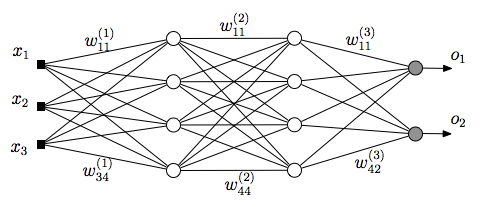
\includegraphics[scale=0.5]{img/MLP}
    \caption{Paveikslėlio pavyzdys}
    \label{img:mlp}
\end{figure}


\section{Eksperimentinio palyginimo rezultatai}
% tablesgenerator.com - converts calculators (e.g. excel) tables to LaTeX
\begin{table}[H]\footnotesize
  \centering
  \caption{Lentelės pavyzdys}
  {\begin{tabular}{|l|c|c|} \hline
    Algoritmas & $\bar{x}$ & $\sigma^{2}$ \\
    \hline
    Algoritmas A  & 1.6335    & 0.5584       \\
    Algoritmas B  & 1.7395    & 0.5647       \\
    \hline
  \end{tabular}}
  \label{tab:table example}
\end{table}

\end{document}
